%Yue -> What do you mean in 3.3? I don't really understand. 

As a group of apprentice engineers, the given task is to optimise a small-scale power transmission system with the objective of minimising the power production cost per hour of the system. In the field of electric power systems operation and planning, the optimal power flow problem also known as the "OPF" is a very useful mathematical optimazition tool. This project is divided into two parts, were the first part (original problem) which treats the OPF is described in chapter 1.1. The second part of the project, further described in chapter 1.3, is an altered version of the original problem were instead an approximation of the OPF is treated.

\subsection{Original problem}
The given small-scale power transmission system is made up of four nodes (1, 2, 3 and 4) which are connected by four links. It is further stated that there are two generators (G1 and G2) located at node 1 and four more generators (G3, G4, G5 and G6) located at node 2. The overall transmission system is illustrated in Figure 1 with the appurtenant components (nodes, links and generators). \\

\begin{figure}[!h]
    \centering
    
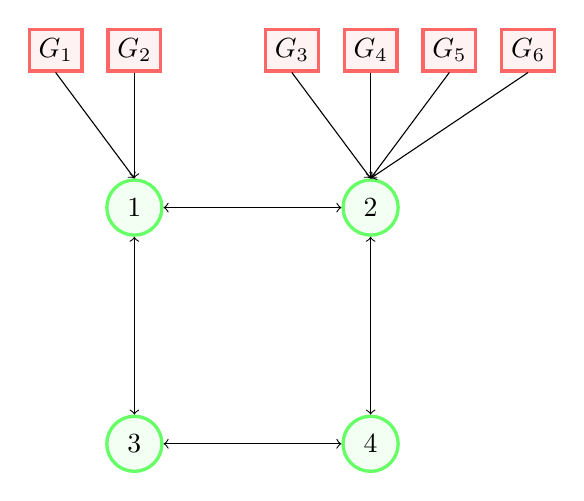
\begin{tikzpicture}[
roundnode/.style={circle, draw=green!60, fill=green!5, very thick, minimum size=7mm},
squarednode/.style={rectangle, draw=red!60, fill=red!5, very thick, minimum size=5mm},
]
%Nodes
\node[roundnode]    (node1)      at (0,0) {1};
\node[roundnode]    (node2)      at (3,0) {2};
\node[roundnode]    (node3)      at (0,-3) {3};
\node[roundnode]    (node4)      at (3,-3) {4};
\node[squarednode]  (gen1)       at (-1,2) {$G_1$};
\node[squarednode]  (gen2)       at (0,2) {$G_2$};
\node[squarednode]  (gen3)       at (2,2) {$G_3$};
\node[squarednode]  (gen4)       at (3,2) {$G_4$};
\node[squarednode]  (gen5)       at (4,2) {$G_5$};
\node[squarednode]  (gen6)       at (5,2) {$G_6$};
 
%Lines
\draw[<->] (node1.east) -- (node2.west);
\draw[<->] (node3.east) -- (node4.west);
\draw[<->] (node1.south) -- (node3.north);
\draw[<->] (node2.south) -- (node4.north);
\draw[->] (gen1.south) -- (node1.north);
\draw[->] (gen2.south) -- (node1.north);
\draw[->] (gen3.south) -- (node2.north);
\draw[->] (gen4.south) -- (node2.north);
\draw[->] (gen5.south) -- (node2.north);
\draw[->] (gen6.south) -- (node2.north);
%\draw[->] (node2.south) .. controls +(down:7mm) and +(right:7mm) .. (node3.east);
\end{tikzpicture}    
    
    \caption{Illustration of power transmission system}
    \label{fig:my_label}
\end{figure}


Furthermore we are given some values on the operational cost and the maximum capacity of the generators which can be seen in Table 2 in the appendix. \\

When it comes to power generation in the given system, one has to consider two types of power generation, active and reactive power. To further explain the difference between the two it is stated that a generator can generate a non-negative amount of active power up to its capacity. For the reactive power however it is assumed that the generator can either absorb or generate some amount of reactive power in the range of plus/minus its capacity. Reactive power is a hard concept to grasp in general and to put it in simple terms it can be seen as a byproduct when generating active power. It is very important to consider the reactive power in a power transmission system as it can cause blackouts and other problems if the voltage goes out of control.  \\

Moreover there is a demand of active power in each node. The demand for each node should be met regardless of any power transmission losses that might occur in the system. The given demands of active power in each node can be seen in Table 3 in the appendix. \\

As for all dynamic systems, there are physical laws that describe the behaviour of our small-scale power transmission system. We will not go through these laws and equations in detail here but instead leave it for the mathematical formulation part. Moreover it is with these equations that we build our model as they describe the power flow and voltage between the nodes.

\subsubsection*{To summarize}
The overall agenda for this part of the project is to formalise the given power flow problem as an optimization problem, create a model in GAMS and then solve the problem. The objective is to minimize the power production cost per hour of the system. From the problem description we were also given some questions that should be answered respectively:

\begin{itemize}
    \item Is the optimization problem we formulated a convex problem or not?
    \item If it was possible to increase the capacity of one generator with 0.1 pu, which generator(s)
    would be the most beneficial to choose?
\end{itemize}

\subsection{Approximation of the OPF}

The second part of the project is to instead of using the OPF, use an approximation of the OPF where one disregards the reactive power all together and further assumes that the voltage amplitude in all nodes are set to 1. One more assumption which is made here is that since the phase angle differences are small it is stated that \textit{$\sin{(\theta_k - \theta_m)} \approx \theta_k - \theta_m$ and $\cos{(\theta_k - \theta_m)} \approx 1$ for all links.} The overall meaning of these assumptions and variables will be further explained in the mathematical formulation part.

\subsubsection*{To summarize}
The task in this part is to based on our results from the first part, determine if this approximation is reasonable. The questions stated in the first part above (1.2) should also be answered here for this approximation of the OPF. Furthermore we were given some questions explicit for this part were the following should be answered:

\begin{itemize}
    \item What is the interpretation of the dual variables associated with the power flow balance
    constraint at each node? Compare the approximate and the nonlinear models.

    \item Investigate the effect of imposing bounds on the active power transmission in the
    links.
    
    \item Can you relate the approximate problem to the nonlinear one and obtain bounds on
    the optimal value of the nonlinear problem?

\end{itemize}


